\documentclass[aspectratio=169,11pt]{beamer}
\usetheme{default}
\setbeamertemplate{navigation symbols}{}
\setbeamertemplate{footline}[frame number]
\setbeamercolor{frametitle}{fg=black!85}
\setbeamercolor{block title}{fg=blue!60!black,bg=blue!8}
\setbeamercolor{block body}{bg=black!3}

\usepackage[T1]{fontenc}
\usepackage{lmodern}
\usepackage{graphicx}
\usepackage{array}
\usepackage{tikz}
\usetikzlibrary{decorations.pathreplacing,arrows.meta}

\newcommand{\sci}[2]{$#1\times10^{#2}$}
\colorlet{hydro}{black!45}
\colorlet{dep}{red!75!black}
\colorlet{cellfill}{blue!5}

\title{Gravity and the pressure limiter}
\subtitle{Follow-up on your sketch}
\author{Keheng Zhu}
\date{11 October 2026}

\begin{document}

%----------------------------------------------------------------------
\begin{frame}
  \titlepage
\end{frame}

%----------------------------------------------------------------------
\begin{frame}{Your point}
  \begin{itemize}
    \item In a column at rest, log pressure is \alert{not flat}:
          from one cell to the next it falls by the hydrostatic amount
          \[
            \Delta \ln p \;=\; -\,\Delta x\,\frac{m_p\, g}{k_B T\,(1+x)}
            \;=\; -\,\frac{\Delta x}{H}
          \]
          {\small ($x$ = ionization fraction, $H$ = pressure scale height)}
    \item So the differences the limiter sees are mostly this built-in fall due to gravity.
    \item Your suggestion: subtract the hydrostatic part, \alert{limit only the departure}
          from balance, then add the hydrostatic part back.
  \end{itemize}
\end{frame}

%----------------------------------------------------------------------
\begin{frame}{What our limiter compares: cell to cell}
  \centering
  \begin{tikzpicture}[x=1.15cm,y=0.92cm,font=\small]
    % cells
    \fill[cellfill] (0,0) rectangle (9,4.2);
    \foreach \xf in {0,3,6,9}
      \draw[dashed,black!50] (\xf,0) -- (\xf,4.2);
    \draw[-{Stealth}] (-0.2,0) -- (9.5,0) node[right] {$x$};
    \node[above] at (1.5,4.2) {cell $i-1$};
    \node[above] at (4.5,4.2) {cell $i$};
    \node[above] at (7.5,4.2) {cell $i+1$};
    \node[below] at (3,0) {face $i-\tfrac12$};
    \node[below] at (6,0) {face $i+\tfrac12$};
    \node[left,rotate=90,anchor=south] at (-0.3,2.1) {$\ln p$};
    % differences between cell centres (staircase)
    \draw[densely dotted,black!60] (1.5,3.3) -- (4.5,3.3);
    \draw[densely dotted,black!60] (4.5,2.2) -- (7.5,2.2);
    \draw[-{Stealth},thick,blue!60!black] (4.5,3.3) -- (4.5,2.32);
    \draw[-{Stealth},thick,blue!60!black] (7.5,2.2) -- (7.5,1.42);
    \node[right,blue!60!black] at (4.55,2.85) {$D_-$};
    \node[right,blue!60!black] at (7.55,1.85) {$D_+$};
    % limited slope in cell i
    \draw[very thick,orange!85!black] (3,2.7) -- (6,1.7);
    \node[orange!85!black,anchor=north east] at (4.3,2.45) {slope};
    % cell-centre values
    \fill (1.5,3.3) circle (2.6pt);
    \fill (4.5,2.2) circle (2.6pt);
    \fill (7.5,1.3) circle (2.6pt);
    % face values
    \draw[thick,fill=white] (3,2.7) circle (3pt);
    \draw[thick,fill=white] (6,1.7) circle (3pt);
    \node (fv) at (4.5,0.75) {face values};
    \draw[-{Stealth},black!70] (fv.north west) -- (3.05,2.55);
    \draw[-{Stealth},black!70] (fv.north east) -- (5.95,1.55);
    % Riemann note
    \node[align=center,font=\footnotesize] (rs) at (7.6,3.45) {Riemann solver here\\(not limited)};
    \draw[-{Stealth},black!70] (rs.west) -- (6.05,3.0);
  \end{tikzpicture}

  \vspace{0.5em}
  {\small The limiter works cell to cell: it compares $D_-$ and $D_+$ and sets the slope inside cell $i$.}
\end{frame}

%----------------------------------------------------------------------
\begin{frame}{What we found in the current code}
  \begin{columns}[T,onlytextwidth]
    \begin{column}{0.53\textwidth}
      \begin{block}{The limiter never cuts the slope}
        \small
        \begin{itemize}
          \item Cells are tiny next to the scale height: about 250 per $H$ in the
                chromosphere, about 1000 in the transition region.
          \item So $D_-/D_+$ for $\ln p$ stays between 0.95 and 1.13 (first 60\,s).
                The limiter only acts below 0.4 or above 2.5.
          \item The imbalance comes from reconstruction and the gravity term
                not cancelling exactly.
          \item It is largest at the top of the transition region
                (around 2149\,km), where $H$ changes fastest:
                the region your sketch marks.
        \end{itemize}
      \end{block}
    \end{column}
    \begin{column}{0.43\textwidth}
      \begin{block}{A bug found on the way}
        \small
        \begin{itemize}
          \item The limiter should be the BATSRUS ``MC3/Koren'' limiter
                (third order on smooth profiles).
          \item Our code had two branches swapped, which made it a
                second-order variant.
          \item Parabola test, face value:\\
                BATSRUS 6.25 (exact), ours 5.917.
          \item \alert{Fixed.}
        \end{itemize}
      \end{block}
    \end{column}
  \end{columns}
\end{frame}

%----------------------------------------------------------------------
\begin{frame}{Your idea, as implemented (prototype)}
  \begin{columns}[T,onlytextwidth]
    \begin{column}{0.62\textwidth}
      \centering
      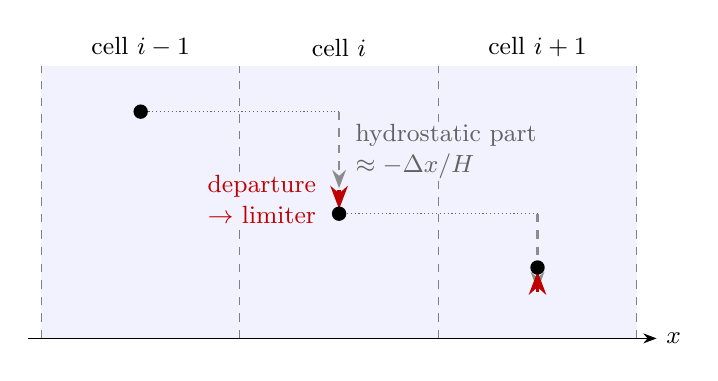
\begin{tikzpicture}[x=0.84cm,y=0.72cm,font=\small]
        \fill[cellfill] (0,0) rectangle (9,4.8);
        \foreach \xf in {0,3,6,9}
          \draw[dashed,black!50] (\xf,0) -- (\xf,4.8);
        \draw[-{Stealth}] (-0.2,0) -- (9.3,0) node[right] {$x$};
        \node[above] at (1.5,4.8) {cell $i-1$};
        \node[above] at (4.5,4.8) {cell $i$};
        \node[above] at (7.5,4.8) {cell $i+1$};
        % staircase guides
        \draw[densely dotted,black!60] (1.5,4.0) -- (4.5,4.0);
        \draw[densely dotted,black!60] (4.5,2.2) -- (7.5,2.2);
        % hydrostatic part (dashed, gray)
        \draw[-{Stealth},thick,dashed,hydro] (4.5,4.0) -- (4.5,2.65);
        \draw[-{Stealth},thick,dashed,hydro] (7.5,2.2) -- (7.5,0.85);
        % departures (red)
        \draw[-{Stealth},very thick,dep] (4.5,2.62) -- (4.5,2.28);
        \draw[-{Stealth},very thick,dep] (7.5,0.82) -- (7.5,1.18);
        % labels
        \node[hydro!70!black,anchor=west,align=left,fill=cellfill,inner sep=1pt] at (4.7,3.3)
             {hydrostatic part\\$\approx -\Delta x/H$};
        \node[dep,anchor=east,align=right,fill=cellfill,inner sep=1pt] at (4.2,2.45)
             {departure\\$\to$ limiter};
        % dots
        \fill (1.5,4.0) circle (2.6pt);
        \fill (4.5,2.2) circle (2.6pt);
        \fill (7.5,1.25) circle (2.6pt);
      \end{tikzpicture}

      \vspace{0.4em}
      {\small Subtract the expected gravitational fall, limit only what is
      left, add the fall back. Use the same fall in the gravity term, so a
      resting atmosphere stays exactly at rest.\par}
    \end{column}
    \begin{column}{0.35\textwidth}
      \small
      \begin{itemize}
        \item Switch \texttt{ISO\_HSE\_RECON=1}, off by default.
        \item Each cell uses its own hydrostatic step; the gravity term
              uses exactly the same step.
        \item Starting state and boundary ghost cells follow the same rule.
        \item Subtlety: the code's gravity differs from nominal $g$ by
              \sci{5}{-8}. With nominal $g$, a tiny uniform sinking
              (\sci{1}{-5}\,m\,s$^{-2}$) remained.
      \end{itemize}
    \end{column}
  \end{columns}
\end{frame}

%----------------------------------------------------------------------
\begin{frame}{How we measure the errors}
  \centering
  \begin{tikzpicture}[x=1cm,y=1cm,font=\footnotesize]
    \def\nc{9}
    \def\w{0.74}
    % ---------------- Result 1 ----------------
    \node[anchor=west,font=\small] at (-0.6,6.85)
      {\textbf{Result 1:} gas at rest, conduction off. Nothing drives it, so the exact answer is \textbf{no motion}.};
    \fill[cellfill] (0,4.9) rectangle (\nc*\w,5.7);
    \draw[black!60] (0,4.9) rectangle (\nc*\w,5.7);
    \foreach \k in {1,...,8} \draw[dashed,black!45] (\k*\w,4.9) -- (\k*\w,5.7);
    % spurious face fluxes and cell speeds (red, random sign)
    \foreach \k/\s in {1/1,2/-1,3/1,4/1,5/-1,6/1,7/-1,8/1}
      \draw[-{Stealth[length=1.6mm]},thick,dep] (\k*\w-0.16*\s,5.98) -- (\k*\w+0.16*\s,5.98);
    \node[anchor=east,dep] at (-0.05,5.98) {$F$};
    \foreach \k/\s in {0/1,1/-1,2/1,3/-1,4/1,5/1,6/-1,7/1,8/-1}
      \draw[-{Stealth[length=1.4mm]},dep!70] (\k*\w+\w/2-0.13*\s,5.3) -- (\k*\w+\w/2+0.13*\s,5.3);
    \node[anchor=east,dep!80] at (-0.05,5.3) {$u$};
    \node[below,black!60] at (0,4.9) {1600\,km};
    \node[below,black!60] at (\nc*\w,4.9) {2153\,km};
    \draw[-{Stealth},black!50] (2.2,4.65) -- (4.4,4.65) node[midway,below] {height};
    \node[anchor=north west,align=left,text width=5.3cm] at (7.25,6.55)
      {\textbf{Spurious mass flux:} largest $|F|$ at any face, before step 1 [kg\,m$^{-2}$\,s$^{-1}$]\\[3pt]
       \textbf{Spurious speed:} largest $|u|$ in any cell at 20\,s [m/s]\\[3pt]
       \textbf{Ideal: 0} (in practice, round-off)};
    \draw[black!25] (-0.6,4.0) -- (12.7,4.0);
    % ---------------- Result 2 ----------------
    \node[anchor=west,font=\small] at (-0.6,3.65)
      {\textbf{Result 2:} evaporation, conduction on, measured at $t=1000$\,s.};
    \fill[cellfill] (0,1.7) rectangle (\nc*\w,2.5);
    \fill[blue!20] (7*\w,1.7) rectangle (\nc*\w,2.5);
    \draw[black!60] (0,1.7) rectangle (\nc*\w,2.5);
    \foreach \k in {1,...,8} \draw[dashed,black!45] (\k*\w,1.7) -- (\k*\w,2.5);
    \foreach \k in {7,8} \draw[-{Stealth[length=1.6mm]},thick,blue!60!black] (\k*\w+0.17,2.1) -- (\k*\w+\w-0.17,2.1);
    \node[above,blue!60!black,align=center] at (8*\w-0.35,2.5) {evaporation speed [m/s]:\\mean $u$, 2130--2150\,km};
    % bottom face highlighted
    \draw[very thick,orange!85!black] (\w,1.6) -- (\w,2.6);
    \node[above,orange!85!black] at (\w,2.6) {bottom face, 1601\,km};
    % zoom of the bottom face: two disagreeing face values
    \draw[orange!85!black,densely dotted] (\w,1.6) -- (1.5,1.25);
    \begin{scope}[shift={(0.3,0)}]
      \draw[black!50] (0,0.05) rectangle (2.4,1.25);
      \draw[thick,orange!85!black] (1.2,0.05) -- (1.2,1.25);
      \draw[very thick] (0.15,0.85) -- (1.2,0.85) node[pos=0.4,above] {$L$};
      \draw[very thick] (1.2,0.45) -- (2.25,0.45) node[pos=0.8,below] {$R$};
      \draw[{Stealth[length=1.3mm]}-{Stealth[length=1.3mm]},dep] (1.32,0.85) -- (1.32,0.45);
      \node[dep,anchor=west] at (1.36,0.75) {jump};
    \end{scope}
    \node[anchor=west,align=left,text width=4.1cm] at (2.85,0.65)
      {The two sides of the face disagree; the Riemann solver turns the jump into extra flux $F_d$.};
    \node[anchor=north west,align=left,text width=5.3cm] at (7.25,3.0)
      {\textbf{Bottom-face error:} split the mass flux at the bottom face,\\[2pt]
       \hspace*{0.3em}$F=\underbrace{\tfrac12(\rho_Lu_L+\rho_Ru_R)}_{F_c\text{: average of } L,R}
         +\underbrace{F_d}_{\text{added for the jump}}$\\[2pt]
       We report $|F_d/F|$. \textbf{Ideal $\approx 0$}: in smooth flow $L$ and $R$ nearly agree.};
  \end{tikzpicture}
\end{frame}

%----------------------------------------------------------------------
\begin{frame}{Result 1: a column at rest stays at rest}
  \framesubtitle{Gas at rest, heat conduction off, 500 and 1000 cells}
  \centering
  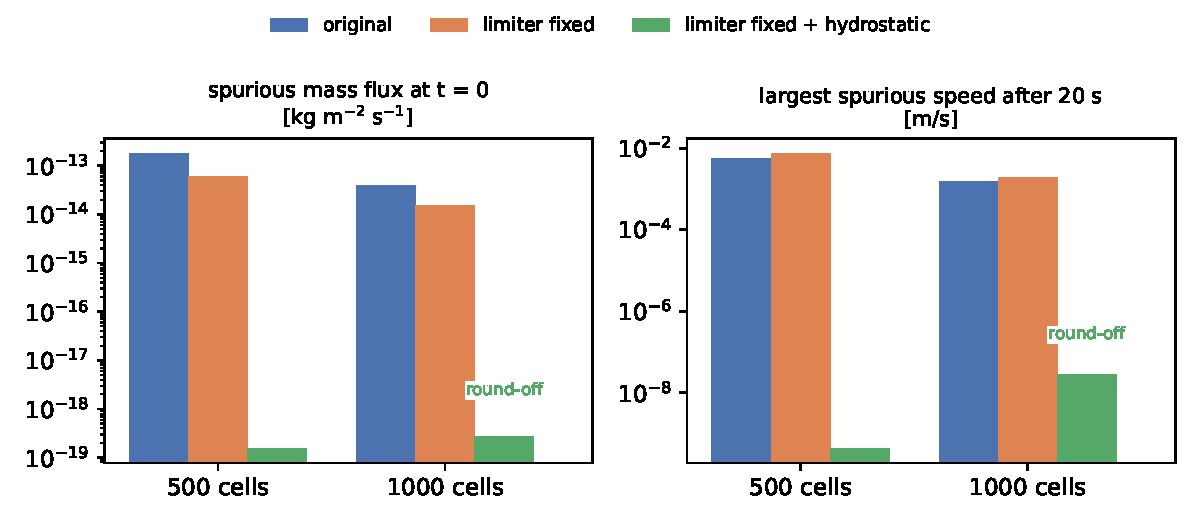
\includegraphics[width=0.66\textwidth]{figures/hse_recon_static_residual.pdf}

  \raggedright\small
  \begin{itemize}
    \item \textbf{Hydrostatic:} at computer round-off at every resolution tried (48 to 2000 cells).
    \item \textbf{Original, limiter fixed:} both quantities shrink about $4\times$ per doubling of cells (second order).
    \item \textbf{Limiter fix alone is mixed:} half the dissipative flux $F_d$ at the bottom face,
          slightly lower spurious speed in the bulk, but about double the spurious speed
          in the top cells (2149--2153\,km) after the first few steps.
  \end{itemize}
\end{frame}

%----------------------------------------------------------------------
\begin{frame}{Result 2: same evaporation, bottom-boundary error removed}
  \framesubtitle{Heat conduction on, 1000\,s, 500 cells (1000 cells look the same)}
  \centering
  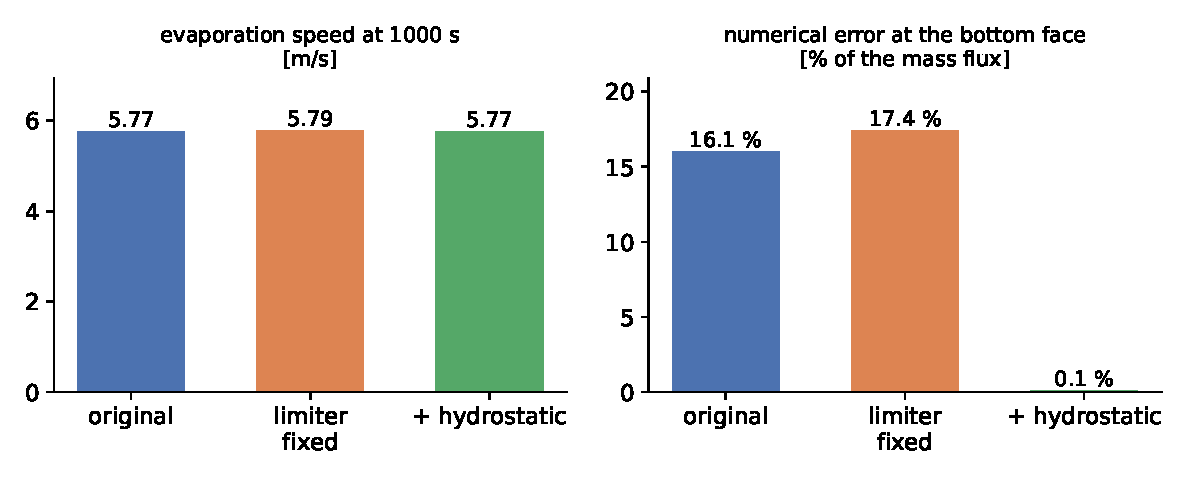
\includegraphics[width=0.74\textwidth]{figures/hse_recon_evaporation_bars.pdf}

  \raggedright\small
  \begin{itemize}
    \item \textbf{Left, the physics:} evaporation speed is the same in all three
          (differences $\le 0.4\,\%$; doubling the cells changes it by 0.9\,\%).
    \item \textbf{Right, the numerics:} at the lowest interior face, 16\,\% of the
          mass flux in the original scheme is numerical dissipation, not physics.
          The hydrostatic version brings this down to \alert{0.1\,\%}.
  \end{itemize}
  \centering\textbf{It removes a numerical error and leaves the answer unchanged.}
\end{frame}

%----------------------------------------------------------------------
\begin{frame}{Summary}
  \begin{itemize}
    \item Our limiter compares cell to cell. On our grid it never cuts the slope;
          the imbalance comes from reconstruction plus gravity not cancelling exactly.
    \item We found and fixed a swapped-branch bug in the limiter.
    \item Your hydrostatic idea works:
      \begin{itemize}
        \item a resting column stays at rest to round-off;
        \item the long-standing bottom-boundary defect goes away (16\,\% $\to$ 0.1\,\%);
        \item evaporation speed barely changes (at most 0.4\,\%).
      \end{itemize}
    \item Limits: exact balance only for a straight field line with constant
          cross-section (our current model). Not the default yet.
  \end{itemize}
\end{frame}

%----------------------------------------------------------------------
\begin{frame}{Questions for you}
  \begin{enumerate}
    \item Should we make the hydrostatic version the default?
    \vspace{0.6em}
    \item Is the per-cell hydrostatic step acceptable, or should we use the
          average temperature of the two cells, as in your sketch?
    \vspace{0.6em}
    \item How high a priority is extending it to a field line whose
          cross-section changes (needs one more term)?
  \end{enumerate}
\end{frame}

%----------------------------------------------------------------------
\begin{frame}{Backup: Result 2 over time}
  \framesubtitle{500 cells solid, 1000 dashed}
  \centering
  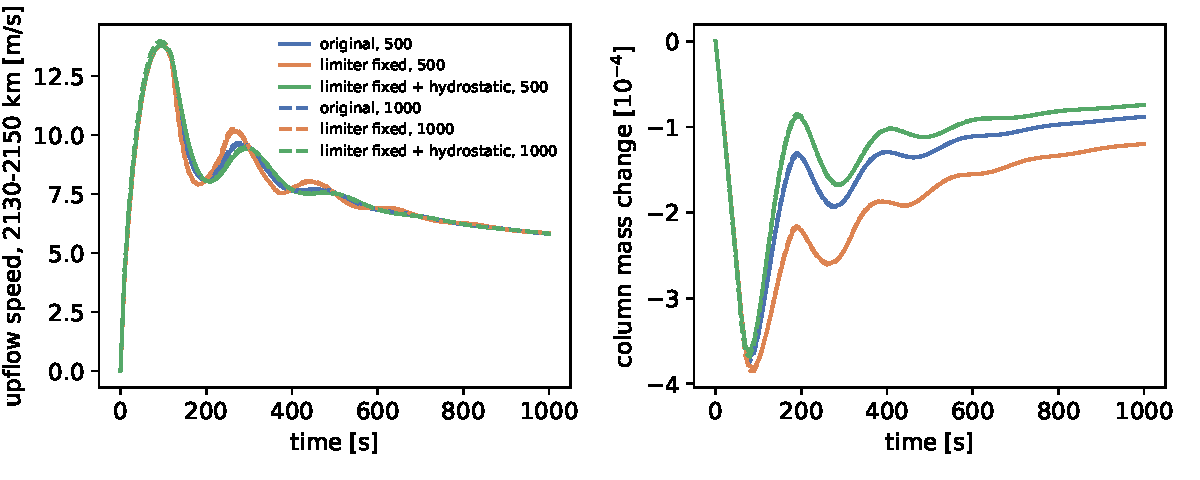
\includegraphics[width=0.73\textwidth]{figures/hse_recon_evaporation.pdf}

  \raggedright\small
  \begin{itemize}
    \item \textbf{Left:} upflow speed in 2130--2150\,km; the schemes differ only in the early oscillations and agree after $\sim$600\,s.
    \item \textbf{Right:} column mass change $M(t)/M(0)-1$, $M=\sum_i\rho_i\,\Delta s_i$. By 1000\,s the original has lost
          \sci{8.8}{-5} of the column; limiter fixed $+36\,\%$, hydrostatic $-16\,\%$.
          The gaps form in the first $\sim$100\,s (start-up near the boundaries)
          and are the same at both resolutions.
  \end{itemize}
\end{frame}

\end{document}
